Given a embedded Giroux domain, this section describes a procedure
to remove its interior and "blow down" the resulting boundary.
We will refer to the procedure as "clean cut-out" of the Giroux domain.

These boundary components are always of the form $B = S^1 \times M$.
Topologically, blowing down is equivalent to simply gluing in $D^2 \times M$.

This operation can be performed in a way that respects the contact structure,
provided that $S^1 \times M$ has a neighborhood
of the form $[0, \epsilon)_s \times S^1_t \times M$ where $\alpha_M + s \d t$
defines a contact form.
In general this holds by \cite[Lemma 5.1]{MNW13} if the boundary components 
are $\xi$-round hypersurfaces, but it is also possible to show the existence 
of that neighborhood directly.

Let $D$ be the disk of radius $\epsilon$ in $\mathbb R^2$. The map 
\[
    \Psi \colon (re^{i\theta} , m) \mapsto (s = r^2, t = \theta, m)
\]
is a diffeomorphism from $(D \setminus \{0\}) \times M$ to 
$(0, \epsilon)_s \times S^1_t \times M$ s.t.
\[
    \Psi^*(\alpha_M + s \d t) = \Psi^*(\alpha_M) + \Psi^*(s\d t) 
    = \alpha_M + r^2 \d \theta,
\]
where the latter contact form can be extended to all of $D^2 \times M$.
In summary: If there is such a neighborhood of $M \times S^1$ as described above, 
we can glue $D \times M$ to $V \setminus B$ to get a new contact manifold 
in which $B$ has been replaced by $M$.

\begin{figure}
    \begin{subfigure}[t]{.293\linewidth}
        \includegraphics[width=\linewidth]{images/blow_down_before.pdf}
        \subcaption{The blue surface is a $\xi$-round boundary surface with (gray) neighborhood}
    \end{subfigure}\hspace*{.1\linewidth}
    \begin{subfigure}[t]{.6\linewidth}
        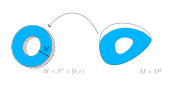
\includegraphics[width=\linewidth]{images/blow_down_topology.pdf}
        \subcaption{Topologically, the blowdown corresponds to gluing $M\times D^2$ 
        on top of the blue surface.}
    \end{subfigure}
    \begin{subfigure}{.9\linewidth}
        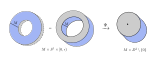
\includegraphics[width=\linewidth]{images/blow_down_contact.pdf}
        \subcaption{Visualization of $\Psi$: The neighborhood of the blue area
        $M \times S^1 \times \{0\}$ on the left is given by $M \times$ the gray annulus.
        In the middle, twist it so that the blue area sits on the inside.
        Applying $\Psi$ is simply retracting the inner circle of the gray annulus to a point.
        The blowdown effectively reduces the inner blue surface $M \times S^1$ to $M = M \times \{0\} \subset M \times D^2$.}
    \end{subfigure}
\end{figure}

Boundary components of Giroux domains are 
$\xi$-round hypersurfaces (\cite[Section 5.3]{MNW13}),
Therefore, after removal of a Giroux domain,
its boundary components can be blown down
These two steps together form the clean cut-out.

In \cite[Section 6]{MNW13}, where the clean cut-out is first introduced,
it is shown that it corresponds to a symplectic cobordism.
The setting there is actually more general: The authors consider a Giroux
domain where already some of the boundary components have been blown down.
In this case, the situation is simpler: The Giroux domain 
$V_- \times S^1 \subset \operatorname{BO}(\Sigma, \dots)$
is directly obtained from the corresponding ideal Liouville domain $V_-$ by 
round contactization.
Its boundary is given by 
\[
    \partial V_- \times S^1 = \Gamma \times S^1.
\]
We want a cobordism from $\operatorname{BO}(\Sigma, \dots)$ to
the same manifold after clean cut-out of $V_- \times S^1$.
Topologically, the cobordism
\[
    W \coloneqq [0,1] \times \operatorname{BO}(\Sigma, \dots) \bigcup_{\{1\} \times \left(V_- \times S^1\right)} V_- \times D^2.
\]
fulfills the requirements: One boundary is simply 
$\operatorname{BO}(\Sigma, \dots)$.
The other boundary is 
\[
    \left[\operatorname{BO}(\Sigma, \dots) \setminus \left(V_- \times S^1\right)\right] 
    \cup_{\Gamma \times S^1} \Gamma \times D^2,
\]
which is homeomorphic to 
$\operatorname{BO}(\Sigma, \dots) \setminus \left(V_- \times S^1\right)$
with blown down boundary, which is exactly the desired clean cut-out.

Next, compute the contact structure on $\operatorname{BO}(\Sigma, \dots) \setminus \left(V_- \times S^1\right)$
with blown down boundary $\partial V_- \times S^1 = \Gamma \times S^1$.

This should be the contact boundary of $V_+ \times D^2$.
Topologically, that makes sense,
\[
    \partial (V_+ \times D^2) = V_+ \times S^1 \cup \partial V_+ \times D^2 = V_+ \times S^1 \cup_{\Gamma \times S^1} \Gamma \times D^2.
\]
However, it is unclear to me why $V_+ \times D^2$ should carry a \underline{symplectic structure}.

It should also be supported by the open book $\operatorname{OB}(V_+, \operatorname{id})$,
which, again, topologically, makes perfect sense, but I don't understand the
\underline{contact side of things}.